\documentclass{beamer}
\usepackage{subfig}

\mode<presentation> {
		\usetheme{Frankfurt}
		\usecolortheme{dolphin}
		\setbeamertemplate{footline}[page number]
}

\title{\huge Vim \\
		\large Making text editing fun and efficient
}

\author{Alec Gibson}
\institute[BlueCat]
{
		BlueCat Networks \\
		\medskip
		\textit{agibson@bluecatnetworks.com}
}
\date{November 24, 2020}

\begin{document}

\begin{frame}
		\titlepage % Print the title page as the first slide
\end{frame}

\begin{frame}
		\frametitle{About This Presentation}
		\begin{itemize}
				\item This presentation was created in Neovim using the Beamer Latex package
				\item The source code is available at: TODO
				\item For discussions about Vim, please post in the company \#vim-geeks slack channel
		\end{itemize}
\end{frame}

\begin{frame}
		\frametitle{Overview}
		\tableofcontents[hideallsubsections]
\end{frame}

\section{What is Vim}
\begin{frame}
		\frametitle{Section Overview}
		\tableofcontents[sections=1]
\end{frame}
\subsection{Introduction}
\begin{frame}
\end{frame}
\subsection{A Brief History of Vim}
\begin{frame}
\end{frame}
\subsection{Who Should Try Vim?}
\begin{frame}
\end{frame}

\section{Vim 101}
\begin{frame}
		\frametitle{Section Overview}
		\tableofcontents[sections=2]
\end{frame}
\subsection{Entering and Exiting Vim}
\begin{frame}
\end{frame}
\subsection{Insert Mode}
\begin{frame}
\end{frame}
\subsection{Normal Mode}
\begin{frame}
\end{frame}
\subsection{Command-Line Mode}
\begin{frame}
\end{frame}
\subsection{Visual Mode}
\begin{frame}
\end{frame}
\subsection{How to Help Yourself}
\begin{frame}
\end{frame}

\section{Power Tools}
\begin{frame}
		\frametitle{Section Overview}
		\tableofcontents[sections=3]
\end{frame}
\subsection{The Jump List}
\begin{frame}
\end{frame}
\subsection{Text Objects}
\begin{frame}
\end{frame}
\subsection{Registers and Macros}
\begin{frame}
\end{frame}
\subsection{Substitute and Global}
\begin{frame}
\end{frame}
\subsection{The Undo Tree}
\begin{frame}
\end{frame}
\subsection{Vimscript}
\begin{frame}
\end{frame}
\subsection{Execute and Normal}
\begin{frame}
\end{frame}

\section{File Navigation}
\begin{frame}
		\frametitle{Section Overview}
		\tableofcontents[sections=4]
\end{frame}
\subsection{Buffers, Windows and Tabs}
\begin{frame}
\end{frame}
\subsection{Argument, Location and Quickfix Lists}
\begin{frame}
\end{frame}
\subsection{Grep and Vimgrep}
\begin{frame}
\end{frame}
\subsection{Cdo, Ldo, Argdo}
\begin{frame}
\end{frame}
\subsection{Finding Files Quickly}
\begin{frame}
		NOTE: discuss fuzzy finder and file tree plugins here
\end{frame}

\section{Configuration}
\begin{frame}
		\frametitle{Section Overview}
		\tableofcontents[sections=5]
\end{frame}
\subsection{Setting Options}
\begin{frame}
\end{frame}
\subsection{Keybindings and Abbreviations}
\begin{frame}
\end{frame}
\subsection{Functions and Custom Commands}
\begin{frame}
\end{frame}
\subsection{Automatic Commands}
\begin{frame}
\end{frame}
\subsection{Plugins}
\begin{frame}
\end{frame}

\section{Links}
\begin{frame}
\end{frame}

\section{Goodbye}
\begin{frame}
		\centerline{\huge All Praise VI VI VI}
		\vspace{0.5cm}
		\centerline{\huge Editor of The Beast}
		\begin{figure}
				\centering
				\subfloat{{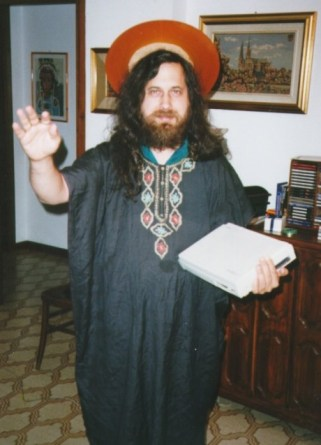
\includegraphics[width=0.3\linewidth]{saintignucius.jpg} }}% Created by Wouter van Oortmerssen
				\qquad
				\subfloat{{
\includegraphics[width=0.3\linewidth]{freebsd-daemon.png} }}% Created by Poul-Henning Kamp under the beer-ware license (https://svnweb.freebsd.org/base/head/share/examples/BSD_daemon/README?view=markup)
		\end{figure}
\end{frame}

\end{document} 
